\graphicspath{{chapters/12/images/}}
\chapter{Heuristics and the genetic algorithm}

``Heuristics is a fancy name for trial-and-error''.

Heuristics mimic natural selection i.e.~follow nature inspired
procedures. At the growing of computational power, they become feasible
ways to solve optimization problems. There are no warranties on the
exactness of the solutions, but often times the results are of high
quality. In addition, heuristic algorithms are easy to implement, are
general and can include \emph{constraints} (even complex ones).
\\
\\
\noindent
Example: timetable for plane departures. Deciding when a plane lands is
not only a function of flight time, we should take into account delays,
passengers, luggages, crew, \ldots{} → constraints. In biological
problems we can include relationship among variables which should be
satisfied, allowing high flexibility.

There are many famous heuristic algorithms:

\begin{itemize}
\tightlist
\item
  simulated annealing: used in physics, match thermal dispersion
\item
  ant colonies: ant are able to solve many problems e.g.~supply chain
\item
  covariance matrix adaptation evolution strategy: performs similarly to
  adaptive MH algorithm
\end{itemize}
\noindent
All these methods have something in common: EVOLUTION STRATEGY.
\\
\\
\noindent
For observing evolution, we require to have a \textbf{population} of
candidate solutions - not only by this method, e.g.~MCMC. We then select
candidates according to their \textbf{fitness function} (objective
function). The changes in the populations occur as results of variations
on the current population.


\subsection{The genetic algorithm}

The genetic algorithm (GA) is a family of evolutionary strategies,
introduced in 1975 by John Holland. It encodes tentative solutions in
chromosomal like structures. Evolution occurs as reproductive
opportunities for the fittest. External variation is introduced through
\emph{mutations}.

\textbf{Fundamental steps}

\begin{itemize}
\tightlist
\item
  encoding of the chromosomes
\item
  generation of an initial population
\item
  fitness evaluation
\item
  parents selection
\item
  reproduction (crossover)
\item
  mutation
\item
  new population
\end{itemize}
\noindent
The process is repeated from the new population to fitness evaluation.
We need to understand how to encode our problem and how the selection of
the mutation and reproduction are performed.


\subsubsection{Chromosome encoding}

\textbf{Chromosome encoding} is performed through bit strings; we have a
long entity \(\theta\) (chromosome) divided into sections (genes).


\subsubsection{Generation of an initial population}

Analogously to the starting points of a multi-start:

\begin{itemize}
\tightlist
\item
  Random
\item
  Latin hypercube
\item
  Orthogonal sampling
\end{itemize}

\subsubsection{Fitness evaluation}

The objective function for the current population could be picked from
known functions e.g.~sum of squares, likelihood or more general
formulations. As long as there is a connection between the fitness
number and candidate selection, the function is fine. MCMC was using one
candidate at a time at each iteration, while gradient methods were
computing the gradient using information from integration. In this case,
the size of the population will determine the number of calls.

\subsubsection{Parent selection}

The parents can be selected through:

\begin{itemize}
\tightlist
\item
  threshold based selection - select best k parameters
\item
  random based selection

  \begin{itemize}
  \item
    Example (similar to Gillespie, we use fitness instead of the
    propensity):

    From \(f^1,\dots,f^N\) compute \(\sum^N_{i=1}f_i=f_0\)

    Generate random number \(j \sim \mathcal{U}(0,1)\)

    Select the smallest k such that \(\sum^k_{i=1}f_i>jf_0\)

    Clone \(\theta^k\) in an intermediate population
  \end{itemize}
\noindent
  ``Roulette selection'', the area of a circle is covered by each
  chromosome fitness proportionally. The idea is to spin the wheel and
  select the chromosome where it stops.
\end{itemize}

\subsubsection{Reproduction}

From the intermediate population we randomly select two individuals
\(u,v\) and a gene for cross over \(t\). We recombine parent chromosomes
and add new offspring to the new population. This procedure is only
inheriting information from the previous generation, we are missing
mutations.

\subsubsection{Mutation}

The offspring may or may not mutate according to a certain probability.
We denote \(p\) the probability that a gene of the new offspring
mutates.

\begin{figure}
\centering
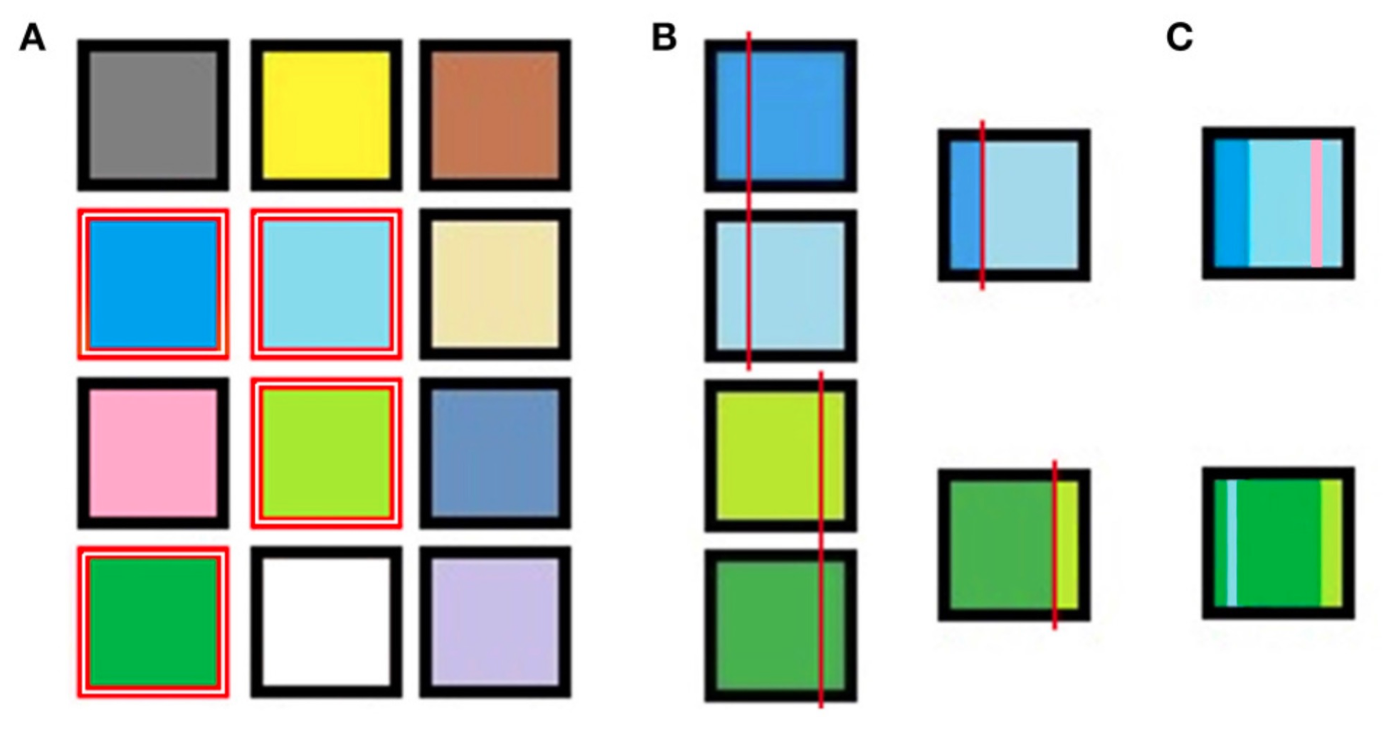
\includegraphics[width=0.5\textwidth]{ga_process.png}
\caption{From Reali et al 2017 - GA procedure example}
\end{figure}


\subsection{Genetic algorithm pseudocode}

\begin{figure}
\centering
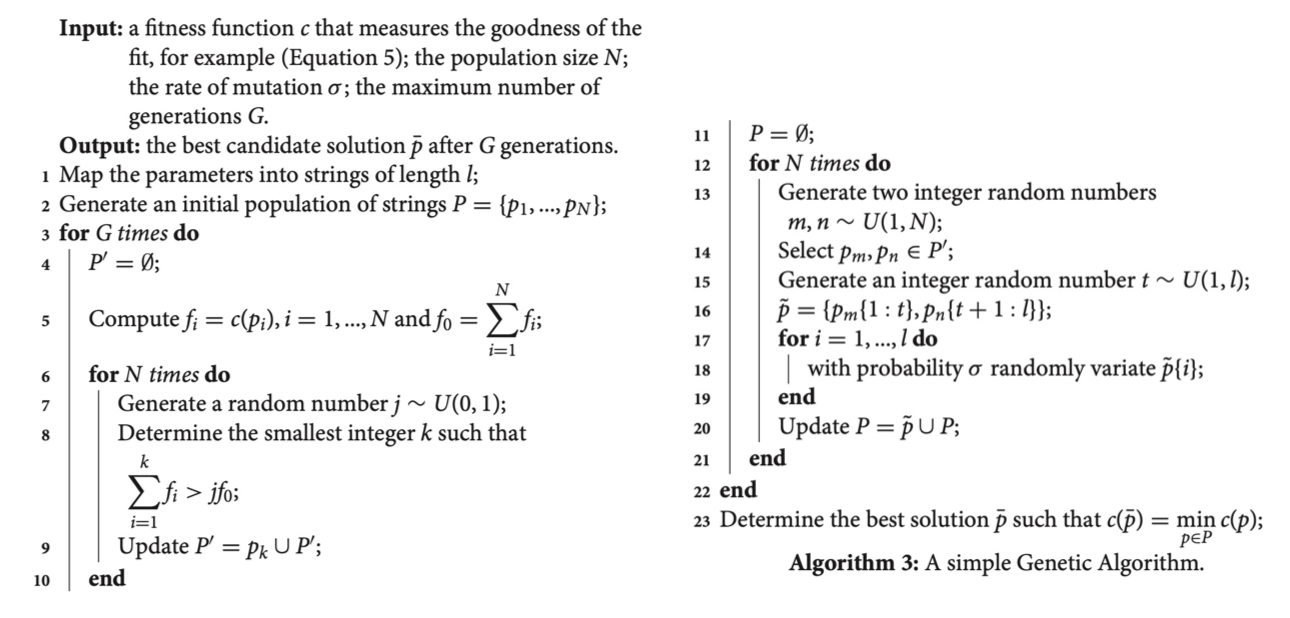
\includegraphics[width=0.8\textwidth]{ga_algo.png}
\caption{From Reali et al 2017 - GA pseudocode}
\end{figure}

\noindent
Observations on specifications:

\begin{enumerate}
\def\labelenumi{\arabic{enumi}.}
\tightlist
\item
  how many times do we go? Here we usually start by defining a number of
  generations
\item
  size of each population, use function to decide
\end{enumerate}

The cost function is as general as possible. GA is sometimes used for
hyperparameters tuning e.g.~we can train a NN inside the algorithm. This
is not feasible with Markov Chains or gradient methods.
\\
\\
\noindent
However, we do not know whether the new generation is better than the
previous one.

\subsubsection{Cons}

It is quite computationally demanding, as for N times we compute the
likelihood/cost/fitness just for selecting new parents. Next, we are not
directly getting direction, the reduction of the fitness function is not
driven by the dimension of the population. Close to the optimum it
converges slowly.

\subsubsection{Pros}

Each one of the computations can be parallelized. Some might argue that
it can be used for everything. It is very general and obtains good
results. \(f\) can vary sometimes; the algorithm can use an obj function
without the constraints, that can be added as penalties after some
generations.
